\documentclass[11pt]{article}
\usepackage{amsmath,amssymb,amsthm,amsfonts,url}
\usepackage{color}
\usepackage{graphicx}
\usepackage{float}
\usepackage{verbatim}
\usepackage[margin=0.8in]{geometry}
\usepackage{subcaption}
\usepackage{indentfirst}
\usepackage[final]{pdfpages}


\usepackage{listings} % For Matlab code insert
\usepackage{color} %red, green, blue, yellow, cyan, magenta, black, white
\definecolor{mygreen}{RGB}{28,172,0} % color values Red, Green, Blue
\definecolor{mylilas}{RGB}{170,55,241}

\parskip 2mm  % Paragraph skip -- the amount of space between paragraphs.

\title{The Mathematics of Gossip}  %title
\author{Ben Hoobler\\ \vspace{2mm} Colorado State University\\May 18, 2018}  %author
\date{}  % let's you fix the date on something -- just switch \today for some other date.
\vspace{-3mm}
\begin{document}
\maketitle  %Inserts title, etc., in the format specified by the documentclass.

%--------------------------------------------------------------------------------------------------------------------% 
\begin{abstract}  
This paper will conduct steady-state analysis and numerical simulations on a modified Susceptible/Infectious/Recovered(SIR) model to investigate the spread of rumors, lies, and misinformation that take place throughout the world today. Maple and MATLAB will be used present a numerical simulations using a Runge-Kutta method and the stability of the dynamical system. The models will be adapted SIR models used to simulate the transmission and spread of the Ebola virus in 2014. Different parameters will be tested such as: susceptibility of ``infection" depending on the source of the information, forgetting and remembering rumors, and the probability that an infected host can realize the rumor is false.
\end{abstract}
%--------------------------------------------------------------------------------------------------------------------% 


%--------------------------------------------------------------------------------------------------------------------% 
\section{Introduction} 
Rumors have had an important role throughout history. Rumors, similar to propaganda, can be viewed as information that is not objective to influence an audience and further an agenda. This is done often by presenting facts selectively to encourage a particular perception, or using loaded language to produce an emotional rather than a rational response to the information that is presented [4]. %Cite this
Due to this, a rumor can spread incredibly fast throughout a network of people and can have dire consequences. The purpose of a rumor may be for slandering others, manipulating situations, causing panic, and so on [1]. A notable event in history caused by a rumor was the Paris Riots in 1750 that caused mass social panic resulting in deadly clashes between Parisians and police.

%In the spring of 1750, a two-day series of riots erupted in Paris when the populace discovered that children were being kidnapped off the streets[2]. Multiple rumors were spread ranging from King Louis XV was kidnapping children to bathe in their blood to cure his leprosy or that the king was kidnapping children to populate far-off French colonies. Neither of these rumors turned out to be true. In reality, the missing children were from an overzealous attempt to control vagrancy. Officers were paid per arrest to bring children to detention houses and were grabbing any children they found wandering the streets, whether they were homeless or not. 
%--------------------------------------------------------------------------------------------------------------------%
\subsection{The Importance of Rumors}
%While the rumors in Paris halted city life for two days and resulted in deadly clashes between civilians and police, there are other dangers due to rumors in the world today. 
With the advancement of the internet and social media, information can spread worldwide in seconds, which can result in physical and economic loss. In 2013, the Associated Press' Twitter account was hacked and sent out a fake tweet stating there was an explosion at the White House that injured President Barack Obama. As the tweet was from a reputable source, it caused the S\&P 500 to lose over \$134 billion within five minutes, causing instability on the world financial market. Once the rumor was proven false the market partly recovered [3].

%The spreading of rumors through a population is very similar to how a epidemic, such as the Ebola virus, spreads through a population. 
The spread of rumors has been described as ``infection of the mind" and their spread is analogous to the spread of an infectious disease, such as Ebola. This analogy is made due to information being passed on from carrier to carrier through a network of contacts [6]. Like a disease, the spreading of rumors can be modeled by differential equations and then numerically simulated for different situations. Studying the function provides information on how to suppress rumors from spreading or successfully spread rumors for malicious intent.   

%--------------------------------------------------------------------------------------------------------------------% 





%--------------------------------------------------------------------------------------------------------------------%
\section{The SIR and ISR Models}   
In the typical SIR model for diseases, the entire population is separated into three groups: $S$ is the number of \textit{susceptible} individuals, $I$ is the number of \textit{infected} individuals, and $R$ is the number of \textit{removed} individuals. The removed individuals are a subset of the infected and susceptible individuals, where they cannot become infected and transmit the disease to others. This could be due to an immunity or have perished from the disease. The standard SIR model for disease spreading is
	\begin{align*}
    \frac{dS}{dt} &= -\lambda I(t)S(t) \\
    \frac{dI}{dt} &=  \lambda I(t)S(t) - \alpha I(t) \\
    \frac{dR}{dt} &=  \alpha I(t),
    \end{align*}
where $\lambda$ is the parameter of infectivity and $\alpha$ is the recovery rate.


For the spreading of rumors, the three groups are: \textit{ignorants} (susceptible individuals), \textit{spreaders} (similar to infected), and \textit{stiflers} (similar to recovered). However, unlike the \textit{recovered} population in the standard SIR equation above, the \textit{stiflers} have a role to play in the rumor spreading.  We define the spreading of rumors to have the following properties: 
\begin{enumerate}
\item If a spreader contacts an ignorant, then the ignorant has a probability $\lambda$ of becoming a spreader.
\item If a spreader makes contact with another spreader or stifler, then the initial spreader has probability $\alpha$ of becoming a stifler.
\item When one or more individuals are informed of a rumor, the spreading process is initialized. 
\item When there are no more spreaders in the population, the rumor is terminated. 

\end{enumerate}
The following equations are for a rumor spreading model, which will be called an ISR model.
	\begin{align}
    \dot{I} = \frac{dI}{dt} &= -\lambda\,\kappa\,I(t)S(t) \\
    \dot{S} = \frac{dS}{dt} &=  \lambda\,\kappa\,I(t)S(t)-\alpha\,\kappa\,S(t) \left[ S(t)+R(t) \right] 
 \\
    \dot{R} = \frac{dR}{dt} &=  \alpha\,\kappa\,S(t) \left[ S(t)+R(t) \right] 
    \end{align}
The variable $\kappa$ is the degree of network reach. For example, the Associated Press has over 12.4 million followers on Twitter. The rumor sent from their hacked Twitter account an extremely high $\kappa$ due to being a reputable sources with an easy access to millions of people. 
We assume that the total population N is constant, therefore $I + S + R = N$. When observing the equations found in the $ISR$ model, it can be seen that $\frac{dS}{dt}$ is a linear combination of $\frac{dR}{dt} - \frac{dI}{dt}$ of equation 1 and 2.
%--------------------------------------------------------------------------------------------------------------------%
\subsection{Stability Analysis of the ISR Model}
As stated above, the given ISR model can be seen as: 	
    \begin{align*}
    \dot{I} &= -\lambda\,\kappa\,IS \\
    \dot{S} &=  \lambda\,\kappa\,IS-\alpha\,\kappa\,S \left( S+R \right) 
 \\
    \dot{R} &=  \alpha\,\kappa\,S \left( S+R \right) 
    \end{align*}
with the initial conditions
\begin{equation*}
I(0) \geq 0, \quad  S(0) \geq 0, \quad  R(0) \geq 0.
\end{equation*}

To find the equilibrium states of the system, we first set $\dot{I}$, $\dot{S}$, and $\dot{R}$ equal to zero and solve the system of equations.
    \begin{align*}
    \dot{I} &= -\lambda\,\kappa\,IS = 0 \\
    \dot{S} &=  \lambda\,\kappa\,IS-\alpha\,\kappa\,S \left[ S+R \right] = 0  
 \\
    \dot{R} &=  \alpha\,\kappa\,S \left[ S+R \right] = 0 
    \end{align*}
Using Maple, the above equations can be easily solved. The first equilibrium point is $\left\{I = I, R = R, S = 0 \right\}$ and the second is when $\left\{I = 0, R = -S, S = S\right\}$. To check the validity of the stability points, we find the eigenvalues of the Jacobian matrix with equilibrium situations. The following matrices are the Jacobian matrix for equations 1-3:
\begin{equation*}
J(I, S, R) =
\begin{bmatrix}
    \frac{\partial \dot{I}}{\partial I}       & \frac{\partial \dot{I}}{\partial S} & \frac{\partial \dot{I}}{\partial R}\\
\noalign{\medskip}\frac{\partial \dot{S}}{\partial I}       & \frac{\partial \dot{S}}{\partial S} & \frac{\partial \dot{S}}{\partial R}\\
\noalign{\medskip}\frac{\partial \dot{R}}{\partial I}       & \frac{\partial \dot{R}}{\partial S} & \frac{\partial \dot{R}}{\partial R}
\end{bmatrix}
=
 \left[ \begin {array}{ccc} -\kappa\,S\lambda&-\lambda\,\kappa\,I&0
\\ \noalign{\medskip}\kappa\,S\lambda&\lambda\,\kappa\,I-\alpha\,
\kappa\, \left( S+R \right) -\alpha\,\kappa\,S&-\alpha\,\kappa\,S
\\ \noalign{\medskip}0&\alpha\,\kappa\, \left( S+R \right) +\alpha\,
\kappa\,S&\alpha\,\kappa\,S\end {array} \right]
\end{equation*}

\begin{equation*}
J(I, R, 0) =
 \left[ \begin {array}{ccc} 0&-\lambda\,\kappa\,I&0
\\ \noalign{\medskip}0&\lambda\,\kappa\,I-\alpha\,\kappa\,R&0
\\ \noalign{\medskip}0&\alpha\,\kappa\,R&0\end {array} \right],
\qquad
J(0, -S, S) =
 \left[ \begin {array}{ccc} -\kappa\,S\lambda&0&0\\ \noalign{\medskip}
\kappa\,S\lambda&-\alpha\,\kappa\,S&-\alpha\,\kappa\,S
\\ \noalign{\medskip}0&\alpha\,\kappa\,S&\alpha\,\kappa\,S\end {array}
 \right] 
\end{equation*}

The eigenvalues of each equilibrium Jacobian matrix are:

\underline{Equilibrium 1}: {$0, 0, I\kappa\lambda - R\alpha\kappa$}

\underline{Equilibrium 2}:{$-\kappa S\lambda, 0, 0$}


A key aspect of dynamical system theory is the following theorem which allows the ability to determine the stability of fixed points.

\newtheorem{theorem}{Theorem}
\begin{theorem}
An equilibrium point $\mathbf{x}$ of the differential equation 1 is stable if all the eigenvalues of $\mathbf{J}$, the Jacobian evaluated at $\mathbf{x}$, have negative real parts. The equilibrium point is unstable if at least one of the eigenvalues has a positive real part.
\end{theorem}



The eigenvalues of the 2nd equilibrium matrix are ($-\kappa S \lambda$, 0, 0). According the to theorem above, if the eigenvalues are all negative real parts, the equilibrium point is stable. For all values of $\kappa, S, \textrm{or} \lambda$, the eigenvalue is going to be negative, which implies stability. The first zero eigenvalue corresponds to the fact that its a 2nd order dynamical system and the other zero eigenvalue is related to the stable center manifold[5] that is the straight line $I + R = 1$ on the $(I, R)$ plane.

\begin{equation*}
\frac{dS}{dt} =  \lambda\,\kappa\,I(t)S(t)-\alpha\,\kappa\,S(t) \left[ S(t)+R(t) \right] > 0
\end{equation*}
\begin{align*}
\lambda I S > \alpha S[S+R] \\
S > \frac{\lambda I}{\alpha} - R
\end{align*}

Furthermore, the spread of a rumor only occurs when $\frac{dS}{dt} > 0$. The rumor will continue to spread until the amount of spreaders is less than $\frac{\lambda I}{\alpha} - R$. Once that threshold is reached, the number of spreaders will quickly decrease to zero and the model will reach equilibrium. In the following sections, the ISR model is numerically simulated and points of equilibrium are found depending on the initial conditions of $\lambda$ and $\alpha$.


%Examining the third eigenvalue and considering the fact that $I + R = 1$ and that $\kappa$ is just a constant give us the following equations where $\frac{\alpha}{(\alpha + \lambda)}$ represents the limit of the rumor spreading efficiency:

%\underline{Case 1}: if $0 < I < \frac{\alpha}{(\alpha + \lambda)}$, the equilibrium point is asymptotically stable.

%\underline{Case 2}: if $\frac{\alpha}{(\alpha + \lambda)} < I < 1$, the equilibrium point is unstable.

 
%--------------------------------------------------------------------------------------------------------------------%





%--------------------------------------------------------------------------------------------------------------------%
\subsection{Numerical Analysis of ISR Model}
In this section, numerical simulations are conducted using MATLAB using a Runge-Kutta method to observe the varying effects that the values of $\lambda$ and $\alpha$ have on the spreading of a rumor. In the following situations, unless noted otherwise, the inital conditions are $I(0) = 0.99$, $S(0) = 0.01$, $R(0) = 0.0$, and $\kappa = 0.6$. The only effect of changing $\kappa$ resulted in the change of time needed for the system to reach equilibrium. As $\kappa$ increases, the time needed for the rumor to propagate decreases. 

%% ISR
\begin{figure}[h!] 
\begin{center}
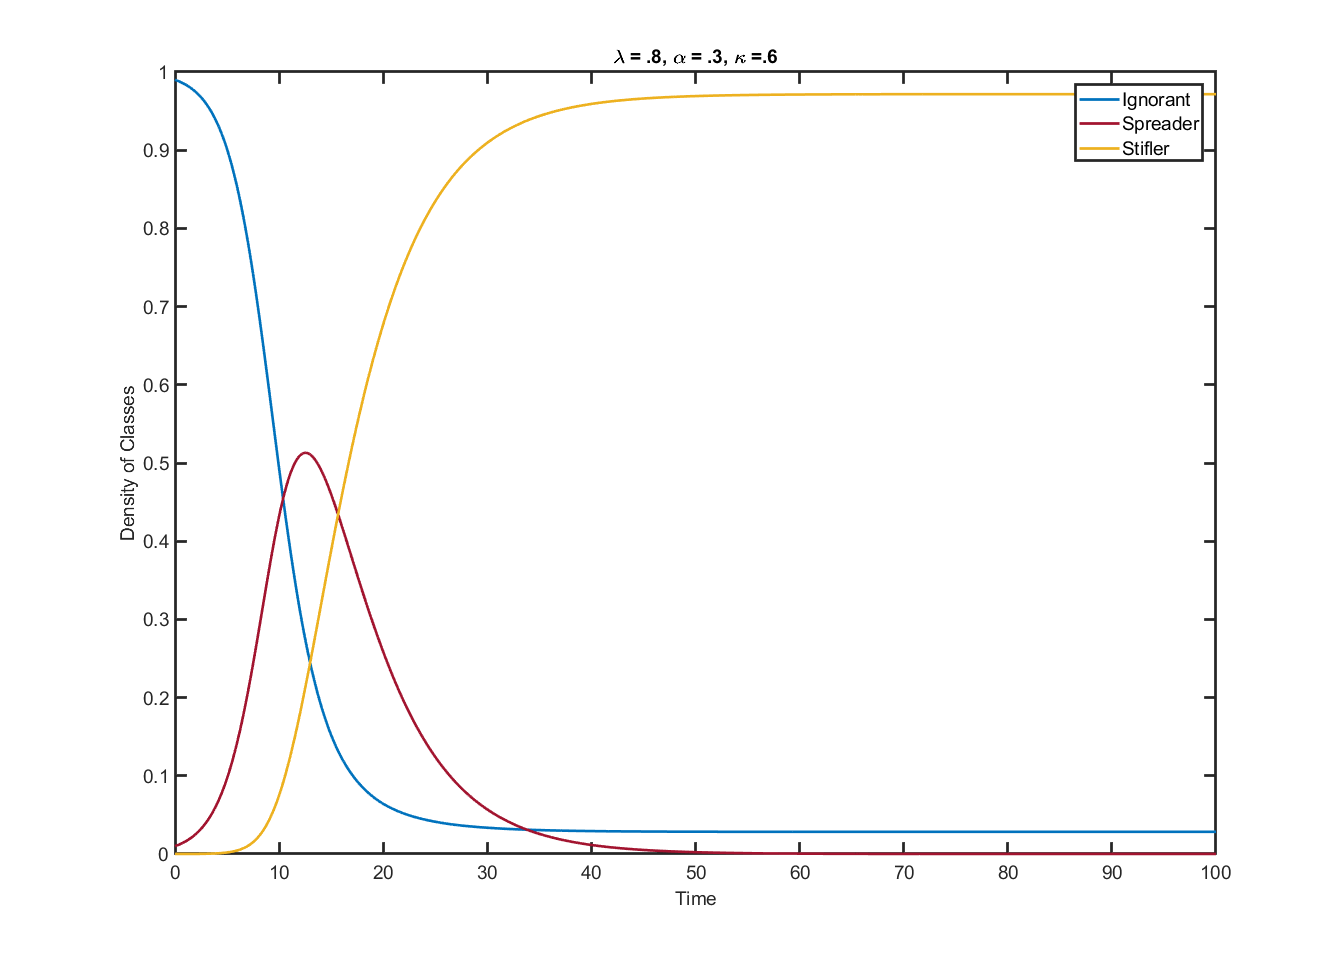
\includegraphics[ width=.75\linewidth]{images/ISR}
\caption{Densities of ignorants, spreaders, and stiflers over time with $\lambda =.8$ and $\alpha = 0.3$} \label{ffc}
\end{center}
\end{figure} 
%%End Figure

Fig. 1 above shows a typical ISR model, where blue represents the \textit{ignorants}, red represents the \textit{spreaders}, and gold represents the \textit{stiflers} who have overcome the rumor. For the following situation, we can see a sharp increase in the number of spreaders as spreaders reaches a peak and thereafter declines. Finally, the number of spreaders is zero and this leads to the termination of the rumor spreading. For the whole process, the number of ignorants always decreases while the number of stiflers always increases until they reach a balance. 

Fig. 2 below shows the densities of ignorants, spreaders, and stiflers over time under different refusing rates $\lambda = 0.2-0.8$ while $\alpha = 0.3$ remains constant. The peak value of $S(t)$ shows the highest density of people spreading the rumor and this can be used to measure the maximum rumor influence. 

%% ISR Vary
\begin{figure}[h!] 
\begin{center}
\includegraphics[height = 7cm, width=\linewidth]{images/all3}
\caption{Density of ignorants, spreaders, and stiflers over time under different refusing rates $\lambda$} \label{ffc}
\end{center}
\end{figure} 
%%End Figure


\subsubsection{$\lambda \approx \alpha$}
Fig. 3 below shows the relationship when $\lambda \approx \alpha$. In this case, the rumor still heavily affects the population. In order to suppress the rumor, $\alpha$ would need to be much larger than $\lambda$. 
%% ISR Vary
\begin{figure}[h!] 
\begin{center}
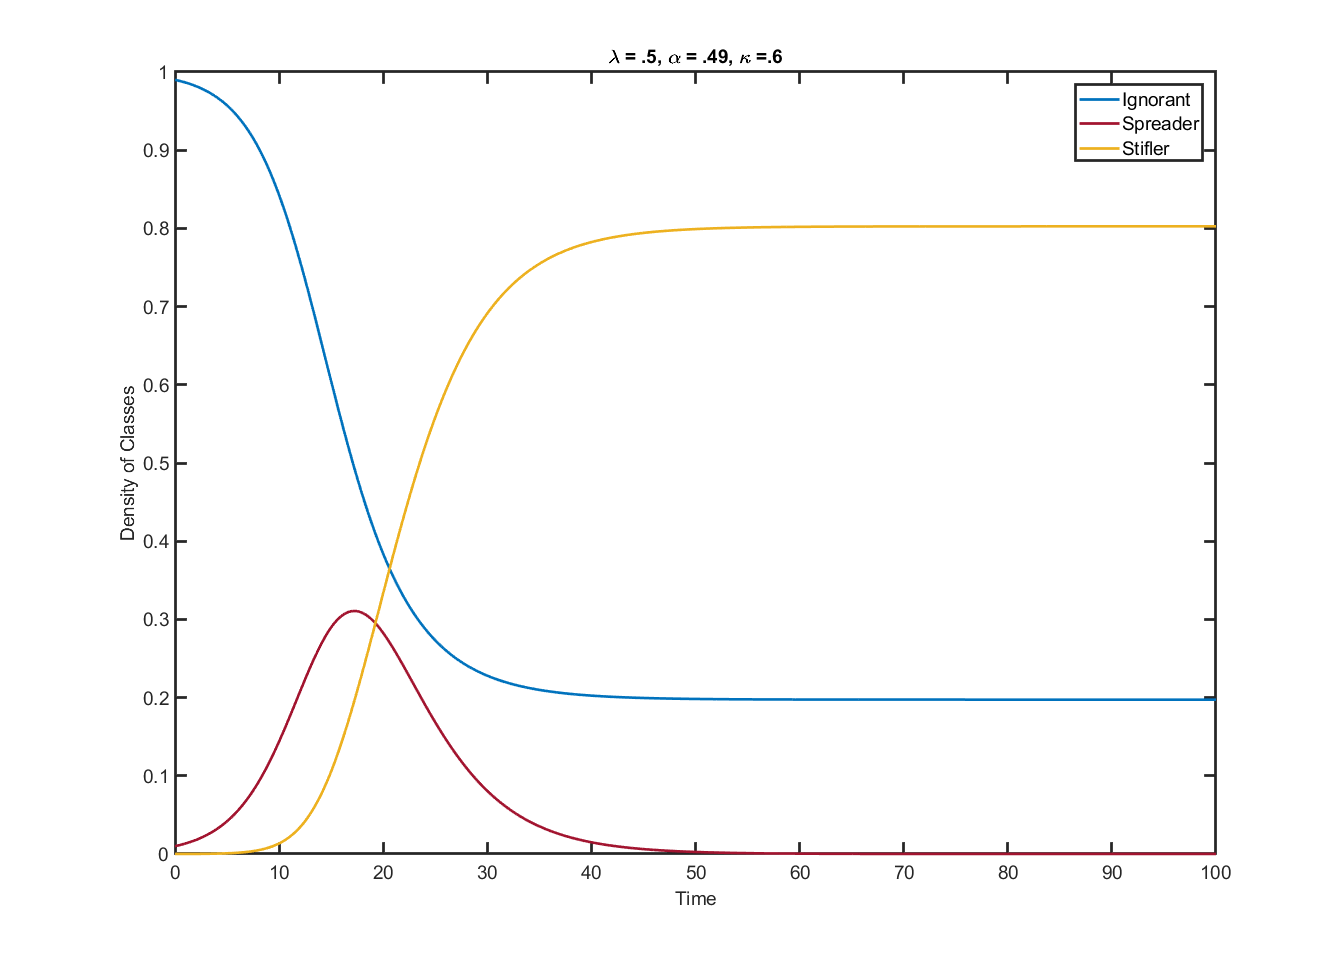
\includegraphics[width=.8\linewidth]{images/Alpha_eq_Kappa}
\caption{Densities of ignorants, spreaders, and stiflers over time with $\lambda =.5$ and $\alpha = 0.49$} \label{ffc}
\end{center}
\end{figure} 
%%End Figure



\subsubsection{$\lambda \ggg \alpha$}
Fig. 4 and 5 show the densities of classes when $\lambda$ is larger than $\alpha$. The larger the $\lambda$, especially the when $\lambda \ggg \alpha$, the larger the maximum influence of the rumor and the longer it takes for the system to reach equilibrium.  

%% ISR Vary
\begin{minipage}{.5\textwidth}
%% ISR Vary
\includegraphics[height = 7cm, width=\linewidth]{images/Lambda8Alpha4.png}
\captionof{figure}{Densities of ignorants, spreaders, and stiflers over time with $\lambda =.8$ and $\alpha = 0.4$} \label{ffc}%%End Figure
\end{minipage}%
\begin{minipage}{.5\textwidth}
%% ISR Vary
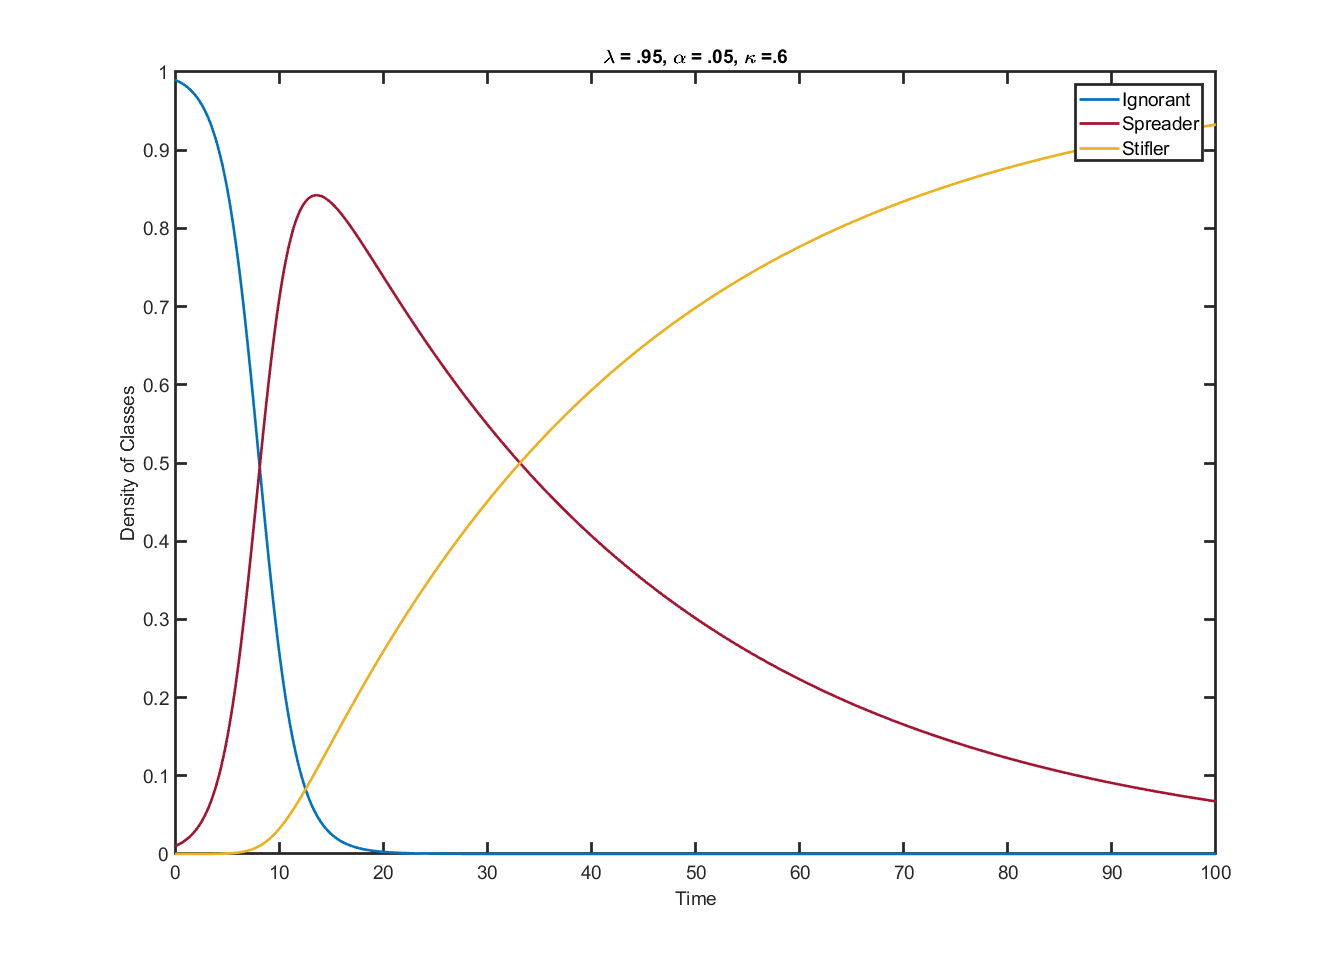
\includegraphics[height = 7cm, width=\linewidth]{images/Lam_gt_Alph}
\captionof{figure}{Densities of ignorants, spreaders, and stiflers over time with $\lambda =.95$ and $\alpha = 0.05$} \label{ffc}
%%End Figure
\end{minipage}%

\subsubsection{$\lambda \lll \alpha$}
In Fig. 6 and 7, $\lambda$ is less than $\alpha$. If more people have the ability to see through the rumor, the maximum rumor influence becomes smaller and the rumor termination time comes earlier. In Fig. 6 the population reaches asymptotic equilibrium where approximately 55\% of the population had heard the rumor before it was suppressed or forgotten. Fig. 7 shows when the stifling rate is much greater than the spreading rate and the rumor barely manages to spread before being suppressed. 

\begin{minipage}{.5\textwidth}
%% ISR Vary
\includegraphics[height = 7cm, width=\linewidth]{images/alpha08}
\captionof{figure}{Densities of ignorants, spreaders, and stiflers over time with $\lambda =.4$ and $\alpha = 0.8$} \label{ffc}%%End Figure
\end{minipage}%
\begin{minipage}{.5\textwidth}
%% ISR Vary
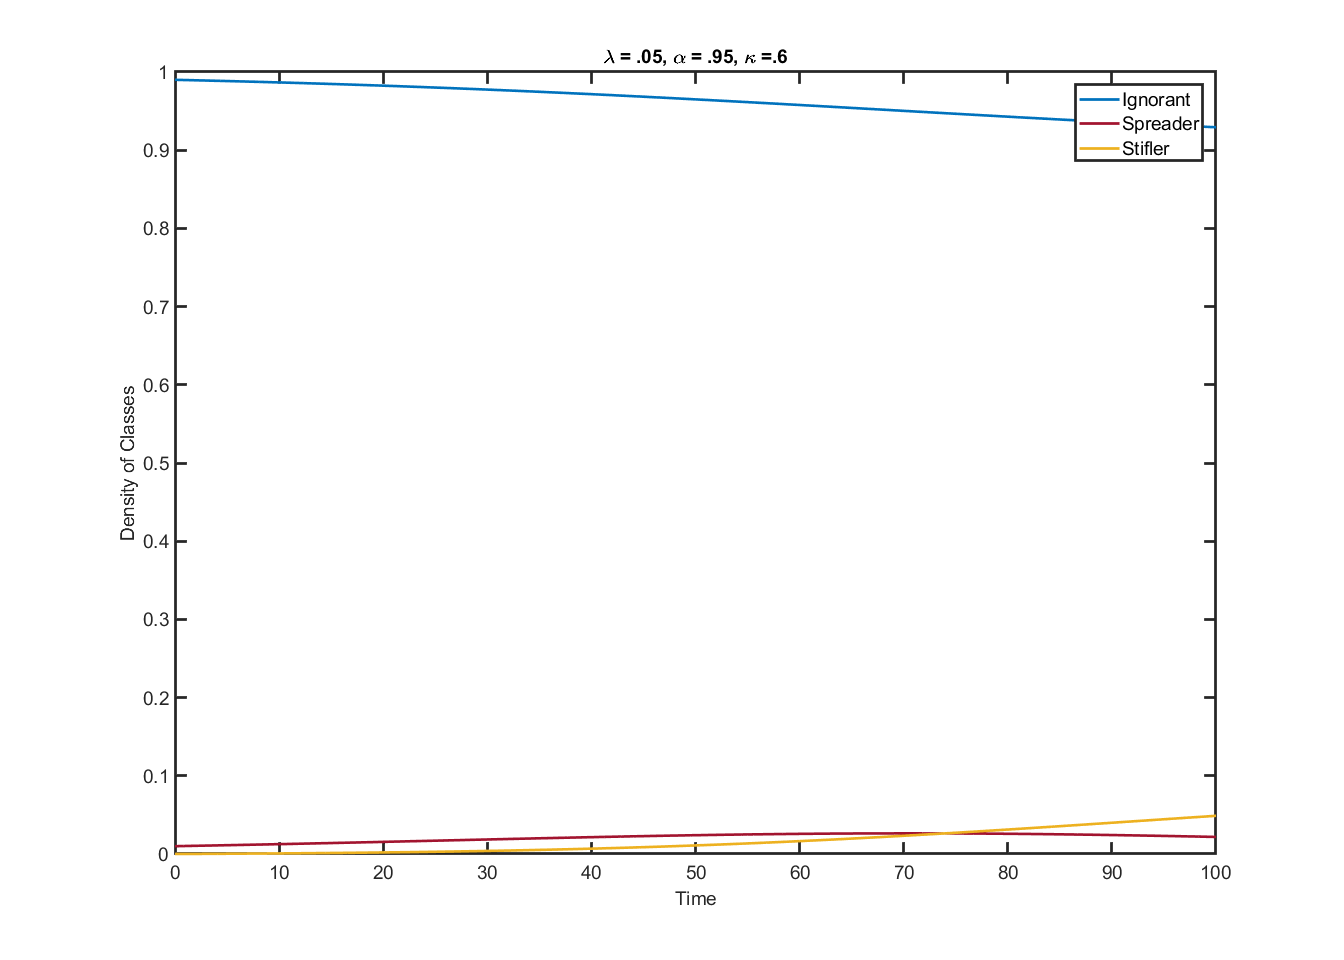
\includegraphics[height = 7cm, width=\linewidth]{images/Alph_gt_Lam}
\captionof{figure}{Densities of ignorants, spreaders, and stiflers over time with $\lambda =.05$ and $\alpha = 0.95$} \label{ffc}
%%End Figure
\end{minipage}%

%--------------------------------------------------------------------------------------------------------------------%
\section{Problems with ISR Model}
There are some issues with the ISR model's functionality. When an ignorant encounters a spreader, the above model fails to represent the situation where an ignorant does not believe the rumor to be true and immediately becomes a stifler. This could be due to the ignorant applying logical reasoning of the situation or mistrusting the credibility of the spreader if they are a known liar, or simply not having interest in the rumor. Education of a particular topic can be easily seen as a ``vaccination" against a rumor. With knowledge gained from education, there is a possibility to transition directly from an ignorant to a stifler when encountering a rumor.

Another issue with the ISR model is the possibility of not spreading the rumor while also not being a stifler. In this case, there would be a new subclass of the ``Infected.'' This can be seen as similar to a disease that has infected a person, but they are not yet infectious to those around them. Because of this new subclass, which will be called \textit{Hibernators}, we introduce a new ISHR Model

%--------------------------------------------------------------------------------------------------------------------%
\section{ISHR Model}
The ISHR model, created by L. Zhao [1], attempts to add new parameters to fix the common problems of the ISR model. The ISR model is extended to include the possibility of an ignorant directly becoming a stifler after hearing the rumor, as well as a new class of ``infected" called \textit{hibernators} are introduced to have the possibility of forgetting and remembering rumors. The new class of hibernators allows for the repeatability of a rumor re-emerging over time. Fig.8 below shows the interaction possibilities of the four classes of the ISHR model. 


%% ISHR Flowchart
\begin{figure}[h!] 
\includegraphics[width=\linewidth]{images/SIHR_Model}
\caption{Flowchart demonstrating the ISHR rumor spreading process} \label{ffc}
\end{figure} 
%%End Figure

The ISHR model can be seen below: 
	\begin{align}
    \frac{dI}{dt} &= (-\lambda + \beta)\kappa I(t)S(t) \\
    \frac{dS}{dt} &= \lambda\kappa I(t)S(t) - \alpha\kappa S(t)[(S(t)+H(t)+R(t)] -\delta S(t) + \xi H(t) + \eta\kappa H(t) S(t) \\
    \frac{dH}{dt} &= \delta S(t) - \xi H(t) - \eta\kappa H(t)S(t) \\
    \frac{dR}{dt} &= \beta\kappa I(t)S(t) + \alpha\kappa S(t)[(S(t)+H(t)+R(t)]
    \end{align}
As the ISHR model is an extension of the ISR model, in certain conditions the original model can be found. When $\beta=0,\delta=0,\xi=0,\eta=0$, the ISHR model becomes the classical ISR rumor spreading model. The rules of the ISHR model can be summarized below:
%% ISHR Model
\begin{figure}[h!] 
\begin{center}
\includegraphics[width=.8\linewidth]{images/SIHR}
\caption{Densities of ignorants, spreaders, hibernators, and stiflers over time with $\lambda$ = 0.8, $\beta$ = 0.2, $\alpha$ = 0.3, $\delta$ = 0.6, $\xi = \eta = 0.5$} 
\label{sihr}
\end{center}
\end{figure}
%%End Figure

\begin{enumerate}
\item If a spreader contacts an ignorant, then the ignorant has a probability $\lambda$ of becoming a spreader.
\item When a spreader contacts an ignorant, the ignorant has a probability $\beta$ of becoming a stifler.
\item A spreader has the probability of becoming a hibernator at a rate $\delta$, which is the forgetting rate of the rumor. A hibernator is a spreader that is not actively spreading the rumor, but has not stifled the rumor. Hibernators can spontaneously become a spreader again at a rate $\xi$, which is the remembering rate. When a hibernator contacts a spreader, the hibernator becomes a spreader with probability $\eta$, which is the wakened remembering rate.
\item If a spreader makes contact with another spreader, hibernator, or stifler, then the initial spreader has probability $\alpha$ of becoming a stifler.
\end{enumerate}

The data from the ISHR model does not act as expected. The model behaves as expected for T = [0,60], but the rapidly increasing stifler population does not act correctly. We should expect the stiflers to plateau at 100\% as $I + S + H + R = 1$. However, in Fig. 9, the stiflers rise to 128.4\% before it starts to plateau. The system of equations should not allow the total population to grow above 100\%. In order study why the model was behaving differently than expected, steady-state analysis was conducted on the new model. 

%--------------------------------------------------------------------------------------------------------------------%
\subsection{Steady-State Analysis of ISHR}
To find the equilibrium states of the system, we first set $\dot{I}$, $\dot{S}$, and $\dot{R}$ equal to zero and solve the system of equations. Then as before, solve for the Jacobian matrix and find the eigenvalues of the equilibrium matrices. 

	\begin{align*}
    \frac{dI}{dt} &= 0 \\
    \frac{dS}{dt} &= 0 \\
    \frac{dH}{dt} &= 0 \\
    \frac{dR}{dt} &= 0
    \end{align*}
    
The equilibrium solutions are the following:

\begin{minipage}{0.48\linewidth}
\begin{align*}
I&= I\\  S&= 0\\ H&= 0 \\  R&= R\\
\end{align*}
\end{minipage}
\begin{minipage}{0.48\linewidth}
\begin{align*}
I &= 0\\ S &= S\\ H &= \frac{\delta S}{(S\eta\kappa+\xi)}\\  R &= \frac{-S(S\eta\kappa+\delta+\xi)}{(S\eta\kappa+\xi)}\\ 
\end{align*}
\end{minipage}




\begin{equation*}
J(I, S , H, R) =
%J0
\left[ \begin {array}{cccc}  \left( -\lambda+\beta \right) \kappa\,S&
 \left( -\lambda+\beta \right) \kappa\,I&0&0\\ \noalign{\medskip}
\lambda\,\kappa\,S&\lambda\,\kappa\,I-\alpha\,\kappa\, \left( S+H+R
 \right) -\alpha\,\kappa\,S-\delta+\eta\,\kappa\,H&-\alpha\,\kappa\,S+
S\eta\,\kappa+\xi&-\alpha\,\kappa\,S\\ \noalign{\medskip}0&-\eta\,
\kappa\,H+\delta&-S\eta\,\kappa-\xi&0\\ \noalign{\medskip}\beta\,
\kappa\,S&\beta\,\kappa\,I+\alpha\,\kappa\, \left( S+H+R \right) +
\alpha\,\kappa\,S&\alpha\,\kappa\,S&\alpha\,\kappa\,S\end {array}
 \right]
\end{equation*}
 

 
 \begin{equation*} %J1
 J(I, 0 , 0, R) =
  \left[ \begin {array}{cccc} 0& \left( -\lambda+\beta \right) \kappa\,
I&0&0\\ \noalign{\medskip}0&\lambda\,\kappa\,I-\alpha\,\kappa\,R-
\delta&\xi&0\\ \noalign{\medskip}0&\delta&-\xi&0\\ \noalign{\medskip}0
&\beta\,\kappa\,I+\alpha\,\kappa\,R&0&0\end {array} \right]
\end{equation*}
 

$J(0, S , \frac{\delta S}{(S\eta\kappa+\xi)}, \frac{-S(S\eta\kappa+\delta+\xi)}{(S\eta\kappa+\xi)}) =$
 \begin{equation*} %J2
 \left[ \begin {array}{cccc}  \left( -\lambda+\beta \right) \kappa\,S&0
&0&0\\ \noalign{\medskip}S\kappa\,\lambda&-\alpha\,\kappa\, \left( S+{
\frac {\delta\,S}{S\eta\,\kappa+\xi}}-{\frac {S \left( S\eta\,\kappa+
\delta+\xi \right) }{S\eta\,\kappa+\xi}} \right) -S\alpha\,\kappa-
\delta+{\frac {\eta\,\kappa\,\delta\,S}{S\eta\,\kappa+\xi}}&-S\alpha\,
\kappa+S\eta\,\kappa+\xi&-S\alpha\,\kappa\\ \noalign{\medskip}0&-{
\frac {\eta\,\kappa\,\delta\,S}{S\eta\,\kappa+\xi}}+\delta&-S\eta\,
\kappa-\xi&0\\ \noalign{\medskip}\beta\,\kappa\,S&\alpha\,\kappa\,
 \left( S+{\frac {\delta\,S}{S\eta\,\kappa+\xi}}-{\frac {S \left( S
\eta\,\kappa+\delta+\xi \right) }{S\eta\,\kappa+\xi}} \right) +S\alpha
\,\kappa&S\alpha\,\kappa&S\alpha\,\kappa\end {array} \right]
\end{equation*}

The eigenvalues of equilibrium 1 were
\begin{enumerate}
\item $\lambda_1 = 0$
\item $\lambda_2 = 0$
\item $\lambda_3 = 1/2\,\lambda\,\kappa\,I-1/2\,R\alpha\,\kappa-\delta/2-\xi/2-1/2\, \\
\sqrt {{I}^{2}{\kappa}^{2}{\lambda}^{2}-2\,IR\alpha\,{\kappa}^{2}
\lambda+{R}^{2}{\alpha}^{2}{\kappa}^{2}-2\,I\delta\,\kappa\,\lambda+2
\,\lambda\,\kappa\,I\xi+2\,R\alpha\,\delta\,\kappa-2\,R\alpha\,\kappa
\,\xi+{\delta}^{2}+2\,\delta\,\xi+{\xi}^{2}}$
\item $\lambda_4 = 1/2\,\lambda\,\kappa\,I-1/2\,R\alpha\,\kappa-\delta/2-\xi/2+1/2\, \\
\sqrt {{I}^{2}{\kappa}^{2}{\lambda}^{2}-2\,IR\alpha\,{\kappa}^{2}
\lambda+{R}^{2}{\alpha}^{2}{\kappa}^{2}-2\,I\delta\,\kappa\,\lambda+2
\,\lambda\,\kappa\,I\xi+2\,R\alpha\,\delta\,\kappa-2\,R\alpha\,\kappa
\,\xi+{\delta}^{2}+2\,\delta\,\xi+{\xi}^{2}}$
\end{enumerate}

No matter the values given to the variables, there will always be at least one eigenvalue that will be positive, which makes equilibrium unstable.




The eigenvalues of equilibrium 2 were 
\begin{enumerate}
\item $\lambda_1 = \kappa\,S\beta-S\kappa\,\lambda$
\item $\lambda_2 = 0$
\item $\lambda_3 = 0$
\item $\lambda_4 = {S}^{2}{\eta}^{2}{\kappa}^{2}+2\,S\eta\,\kappa\,\xi+\delta\,\xi+{\xi}^
{2}$
\end{enumerate}
 When numerically calculating the eigenvalues of equilibrium 2, the eigenvalues were complex with negative real parts:
\begin{itemize}
\item $\lambda_1 =$ $-2.79453109958139\cdot 10^{-17} + i 1.27433158109030\cdot 10^{-10}$
\item $\lambda_2 =$ $-2.79453109958139\cdot 10^{-17} - i 1.27433158109030\cdot 10^{-10}$
\item $\lambda_3 =$ $-1.09980239520000$
\item $\lambda_4 =$ $-0.00120000000000$
\end{itemize}  
Since all the eigenvalues were not real, negative values, I was unable to conclude that the ISHR model will converge to a stable equilibrium. 

%--------------------------------------------------------------------------------------------------------------------%


%--------------------------------------------------------------------------------------------------------------------%
\section{Conclusions and Future Work}
In this paper, the goal was to model the complexity of rumors within a population based on SIR epidemic models. In today's world with the power of social media, the growth of rumors can be extremely tricky to inhibit. As the spread of rumors can be seen as as ``infection of the mind" or ``thought contagion", their spread is analogous to the spread of an infectious disease. The ISR model did an acceptable job to show how quickly a rumor can propagate. Steady-state analysis was successfully conducted on the system of differential equations to show that the system has a stable equilibrium. The model isn't without its flaws, and a new model was considered to add more realistic factors to rumor spreading model to make it closer to real life. The more complex ISHR model was unsuccessful in demonstrating the propagation of rumors.

I would be curious to look at and model a data set of rumors from Twitter from a particular incident, such as the Boston Marathon Bombings. During that time, tens of thousands of tweets were sent and retweeted containing false information, such as how many bombs were set off, who the attackers were, ect. Then analyze what tweets had a high believability rate $\lambda$ and be able to see if a predicted model would closely match the real model from the data set. 
%--------------------------------------------------------------------------------------------------------------------%



%--------------------------------------------------------------------------------------------------------------------%

\section{Acknowledgments}
Special thanks to Dr. Patrick Shipman for his guidance and encouragement to continue and strive to make this project better. Also to Joshua de Jong for his ever-present willingness to help me through my coding errors. I also wanted to thank L. Zhao and J.R Peiqueira for their ISHR and ISR models, respectively. 

\begin{thebibliography}{99}
\bibitem{bert_real} L. Zhao, J. Wang, Y. Chen, Q. Wang, J. Cheng, and H. Cui, ``ISHR Rumor Spreading Model in Social Networks,” \textit{Physica A: Statistical Mechanics and its Applications}, Vol. 391, No. 7, 2444-2453, 2012.
\bibitem{bert_real} A. Farge, \textit{Vanishing Children of Paris: Rumor and Politics Before the French Revolution}. Cambridge: Harvard Univ Press, 1993.
\bibitem{bert_real} P. Domm, ``False Rumor of Explosion at White House Causes Stocks to Briefly Plunge," CNBC, 2013. 
\bibitem{bert_real} J. R. Piqueira, ``Rumor Propagation Model: An Equilibrium Study," \textit{Mathematical Problems in Engineering}, vol. 2010, pp. 1–7, 2010.
\bibitem{bert_real}  J. Guckenheimer, P. Holmes, \textit{Nonlinear Oscillations, Dynamical Systems, and Bifurcations of Vector
Fields}, vol. 42 of Applied Mathematical Sciences, Springer, New York, NY, USA, 1983.
\bibitem{bert_real} S. Funk, E. Gilad, C. Watkins, and V. A. A. Jansen, ``The spread of awareness and its impact on
epidemic outbreaks,” \textit{Proceedings of the National Academy of Sciences of the United States of America},
vol. 106, no. 16, pp. 6872–6877, 2009.
\bibitem{bert_real} M. R. Roussel, \textit{Stability Analysis for Ordinary Differential Equations}. Calgary, Canada: ULETH, 2005.
%\bibitem{} S. A. Thomas, ``Lies, Damn Lies, And Rumors: An Analysis Of Collective Efficacy, Rumors, And Fear In The Wake Of Katrina," \textit{Sociological Spectrum}, vol. 27, no. 6, pp. 679–703, 2007.

\end{thebibliography}

\newpage
%--------------------------------------------------------------------------------------------------------------------%
\lstset{language=Matlab,%
    %basicstyle=\color{red},
    breaklines=true,%
    morekeywords={matlab2tikz},
    keywordstyle=\color{blue},%
    morekeywords=[2]{1}, keywordstyle=[2]{\color{black}},
    identifierstyle=\color{black},%
    stringstyle=\color{mylilas},
    commentstyle=\color{mygreen},%
    showstringspaces=false,%without this there will be a symbol in the places where there is a space
    numbers=left,%
    numberstyle={\tiny \color{black}},% size of the numbers
    numbersep=9pt, % this defines how far the numbers are from the text
    emph=[1]{for,end,break},emphstyle=[1]\color{red}, %some words to emphasise
    %emph=[2]{word1,word2}, emphstyle=[2]{style},    
}
\section*{MATLAB Code}
\lstinputlisting{ISR_Model.m}

\newpage

\lstinputlisting{images/SIHR.m}

\newpage

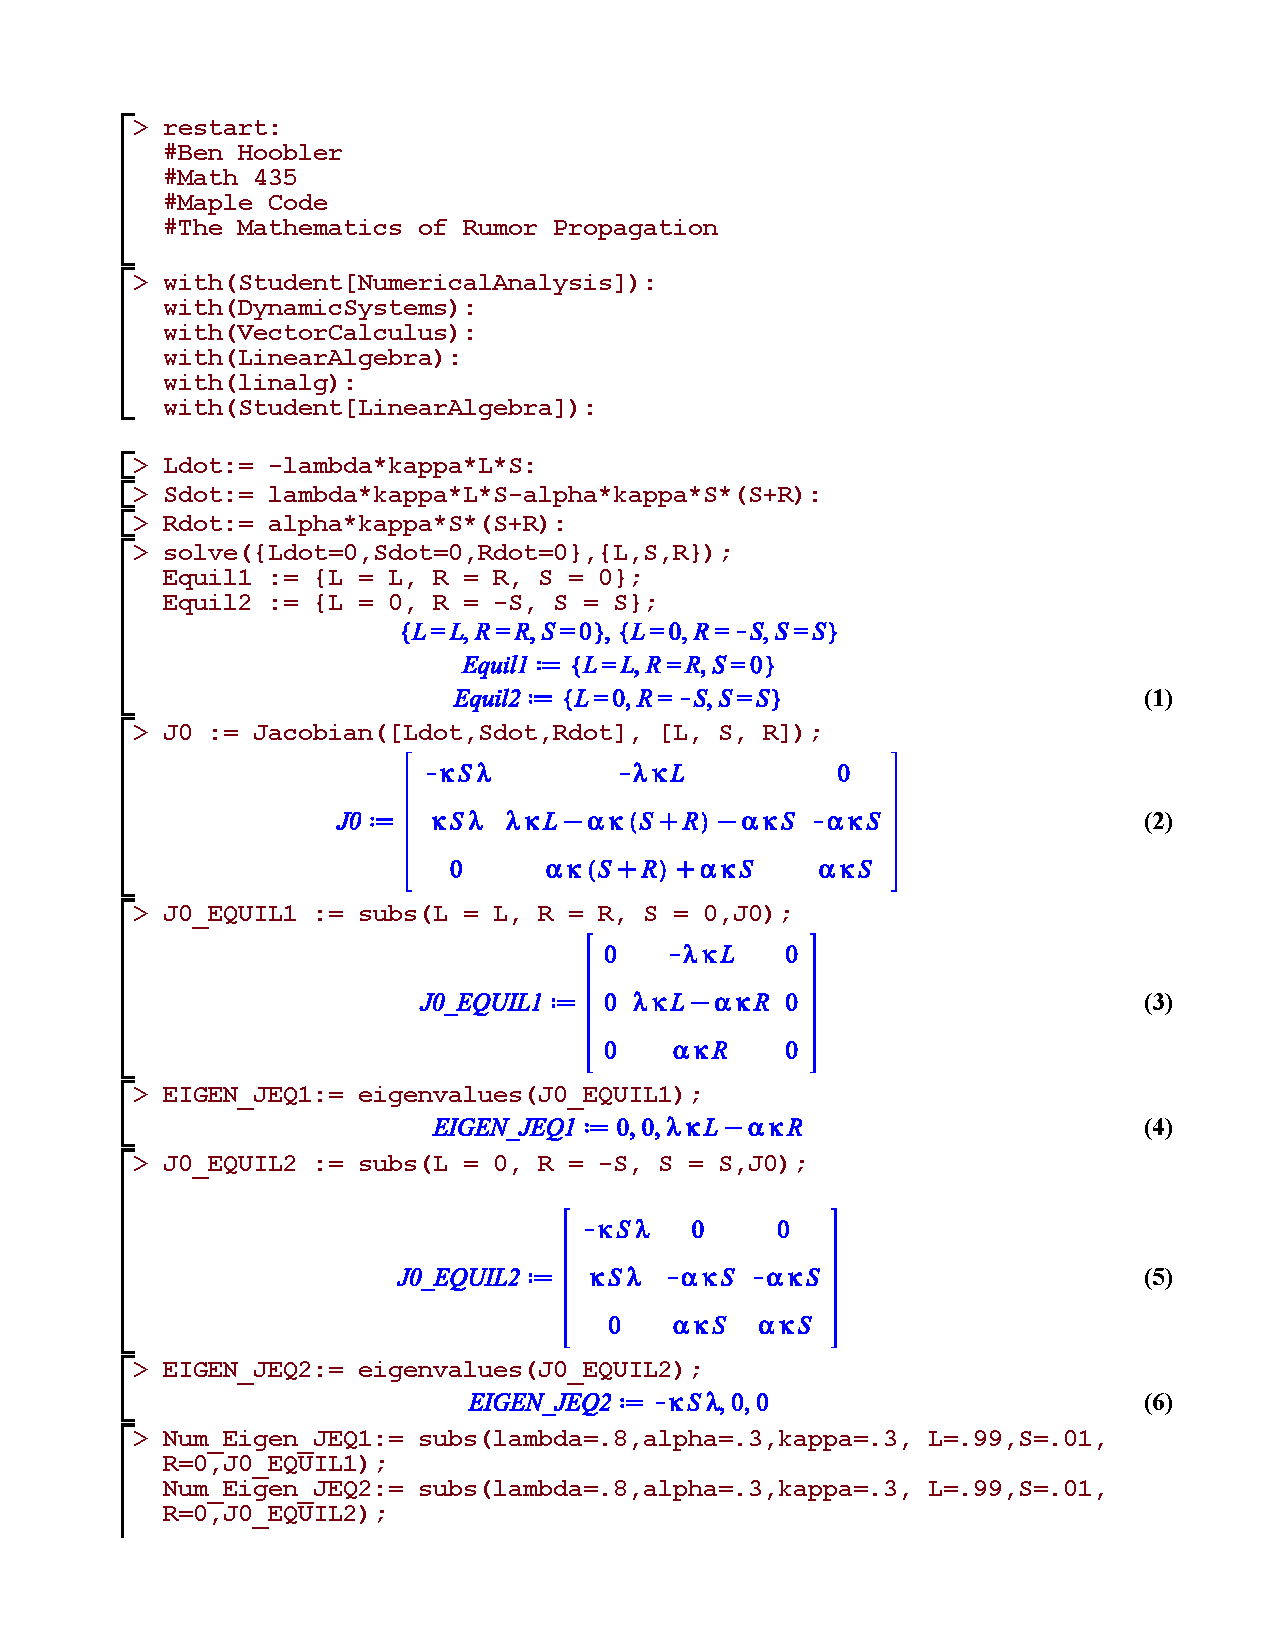
\includepdf[pages=-]{SIR.pdf}
%--------------------------------------------------------------------------------------------------------------------%



\end{document}
